\documentclass[11pt]{article}

\usepackage[margin=1in]{geometry}
\usepackage{booktabs}
\usepackage{tabularx}
\usepackage{array}
\usepackage{amsmath}
\usepackage{graphicx}
\usepackage[font=small,labelfont=bf]{caption}
\usepackage{hyperref}

\title{Collapse-Aware Self-Update for Resource-Limited Medical Language Models}

\author{
Zhequan Hu\textsuperscript{1} and Xingang Bi\textsuperscript{1,*}\\
\textsuperscript{1}Department of Urology, National Cancer Center / Cancer Hospital,\\
Chinese Academy of Medical Sciences and Peking Union Medical College, Beijing, China\\
\textsuperscript{*}Correspondence: \texttt{bixingang@csco.org.cn}
}

\date{}

\begin{document}
\maketitle

\begin{abstract}
Small language models are attractive for medical question answering (QA) under limited compute, but their apparent accuracy can hide a more basic failure mode: answer collapse, where a model repeatedly predicts a dominant label while underusing the answer space. This paper studies task-driven self-update as a lightweight way to recalibrate such behavior. We define self-update operationally as supervised LoRA adaptation on a 44,978-example multi-task medical QA replay mixture built from PubMedQA, MedMCQA, and MedQA, and evaluate Qwen2.5-Instruct models at 0.5B, 1.5B, and 3B parameters across three random seeds. Rather than reporting accuracy alone, we introduce a collapse-aware benchmarker that jointly tracks accuracy, macro-F1, dominant-label rate, normalized prediction entropy, collapse flags, non-model label baselines, frozen-model baselines, and paired McNemar tests.

Across all model scales and tasks, full45k self-update removes collapse in every seed. On PubMedQA, the 0.5B model improves from 0.210 frozen accuracy to 0.650 $\pm$ 0.046 after self-update, while collapse decreases from 1/1 to 0/3 runs. The 1.5B model obtains the best PubMedQA result, reaching 0.690 $\pm$ 0.010 accuracy and 0.584 $\pm$ 0.040 macro-F1. On MedMCQA and MedQA, the 3B model is strongest and highly stable, reaching 0.583 $\pm$ 0.003 and 0.566 $\pm$ 0.002 accuracy, respectively. Paired tests show significant gains for the 0.5B and 3B models across all three tasks and seeds, and for the 1.5B model on MedMCQA and MedQA. These findings suggest that lightweight weight updates can mitigate answer collapse and recalibrate prediction distributions, while also showing that scaling alone does not guarantee stable medical QA behavior.
\end{abstract}

\section{Introduction}

Medical question answering is a demanding setting for language models: tasks differ in answer format, label priors, domain knowledge, and reasoning requirements. Large proprietary systems can often improve through scale, prompting, retrieval, or instruction tuning, but these options are less accessible in resource-limited settings. Small and mid-sized open-weight language models therefore remain important for practical medical NLP research. Yet evaluating such models by accuracy alone can be misleading. A model may obtain non-trivial accuracy by overpredicting a frequent label, while failing to cover clinically meaningful alternatives.

We focus on this failure mode as \emph{answer collapse}: a prediction distribution becomes dominated by one label, or leaves much of the answer space unused. In PubMedQA, this can appear as always answering ``yes'' or ``maybe''; in multiple-choice medical QA, it can appear as repeatedly selecting a single option such as A. Collapse is not merely a cosmetic distributional artifact. It depresses macro-F1, reduces answer-space coverage, and can make an apparently reasonable accuracy number brittle.

This paper asks whether lightweight weight updates can mitigate answer collapse in resource-limited medical language models. We call this setting \emph{task-driven self-update}: the model is updated through LoRA adapters using a multi-task medical QA replay mixture, and the resulting behavior is compared against the same model in its frozen state. The term self-update is used operationally rather than anthropomorphically: the model does not autonomously design its own training objective, but its downstream behavior changes through a small trainable weight component exposed to task evidence.

Our study uses Qwen2.5-Instruct models at 0.5B, 1.5B, and 3B parameters. We train LoRA adapters on a 44,978-example replay mixture built from PubMedQA, MedMCQA, and MedQA, then evaluate frozen and updated models on PubMedQA test100, MedMCQA val1000, and MedQA test1273. Each full45k condition is run with three seeds. We supplement accuracy with macro-F1, dominant-label rate, normalized entropy, collapse flags, non-model baselines, and paired McNemar tests.

The contributions are:
\begin{enumerate}
    \item We formulate a collapse-aware evaluation protocol for medical QA self-update, combining standard accuracy with macro-F1, dominant-label rate, normalized entropy, and explicit collapse flags.
    \item We provide a three-task, three-scale, three-seed study of LoRA-based self-update under limited compute.
    \item We show that full45k task-driven self-update removes collapse across all tested model scales and tasks.
    \item We find that scaling alone is insufficient: frozen 1.5B and 3B models still collapse on PubMedQA, and the strongest PubMedQA result comes from 1.5B rather than 3B.
\end{enumerate}

\section{Related Work}

\paragraph{Medical question answering.}
PubMedQA evaluates yes/no/maybe answers to biomedical research questions derived from PubMed abstracts \cite{jin2019pubmedqa}. MedMCQA is a large multi-subject multiple-choice benchmark based on medical entrance exam questions \cite{pal2022medmcqa}. MedQA is derived from professional medical board exams and is widely used for USMLE-style evaluation \cite{jin2020medqa}. These datasets differ in label space and question format, making them useful for studying whether adaptation improves general medical QA behavior or merely exploits a single task's label distribution.

\paragraph{Parameter-efficient adaptation.}
LoRA freezes the base model and injects trainable low-rank matrices into model layers, substantially reducing adaptation cost relative to full fine-tuning \cite{hu2021lora}. This is particularly attractive when experiments must run on consumer-grade GPUs. We use LoRA not as a new optimization method, but as a controlled mechanism for measuring how a lightweight weight update changes collapse behavior.

\paragraph{Open-weight small language models.}
Qwen2.5 provides a family of open-weight instruction-tuned models across multiple scales \cite{qwen2025qwen25}. This lets us evaluate whether answer collapse is simply solved by increasing model size. Our results suggest that size helps for MedMCQA and MedQA but does not monotonically improve PubMedQA after self-update.

\section{Methods}

\subsection{Task-Driven Self-Update}

We define task-driven self-update as follows. Given a pretrained instruction-tuned language model $M_\theta$, we freeze the base parameters $\theta$ and train LoRA parameters $\phi$ on a medical QA replay mixture. The updated model is $M_{\theta,\phi}$, where only $\phi$ is learned. The goal is not to claim autonomous model improvement, but to test whether a lightweight weight change can recalibrate answer-space behavior.

The replay mixture, denoted full45k, contains 44,978 training examples. It combines PubMedQA with repeated sampling, 30k MedMCQA examples, and 10k MedQA examples. We use this mixture to expose the model to both yes/no/maybe and four-option medical QA formats. Evaluation is performed separately on PubMedQA test100, MedMCQA val1000, and MedQA test1273.

\subsection{Models and Training}

We evaluate Qwen2.5-Instruct models with 0.5B, 1.5B, and 3B parameters. For each model, we first run frozen evaluation. We then train LoRA adapters for one epoch on the full45k replay mixture using seeds 42, 43, and 44. LoRA rank is 8, alpha is 16, dropout is 0.05, and the learning rate is $2\times 10^{-4}$. LoRA is applied to attention projection modules and feed-forward projection modules: \texttt{q\_proj}, \texttt{k\_proj}, \texttt{v\_proj}, \texttt{o\_proj}, \texttt{gate\_proj}, \texttt{up\_proj}, and \texttt{down\_proj}.

The 0.5B model uses maximum sequence length 1536 and has 4.40M trainable LoRA parameters. The 1.5B model uses maximum sequence length 1024 and has 9.23M trainable parameters. The 3B model uses maximum sequence length 768 and has 14.97M trainable parameters. Gradient checkpointing is enabled for 1.5B and 3B runs. All experiments were run on a single NVIDIA GeForce RTX 5060 Ti with 16GB VRAM.

\subsection{Collapse-Aware Benchmarker}

For each task, let $\mathcal{Y}$ be the task label set, and let $p(y)$ be the empirical frequency of predicted label $y$. We compute:
\begin{align}
d &= \max_{y \in \mathcal{Y}} p(y),\\
H_{\mathrm{norm}} &= -\frac{\sum_{y\in\mathcal{Y}} p(y)\log p(y)}{\log |\mathcal{Y}|}.
\end{align}
Here $d$ is the dominant-label rate and $H_{\mathrm{norm}}$ is normalized prediction entropy. A run is flagged as collapsed if $d \geq 0.80$ or if the number of missing predicted labels is at least $\max(1,\lfloor |\mathcal{Y}|/2 \rfloor)$.

We report accuracy and macro-F1 alongside these collapse metrics. Macro-F1 is important because a collapsed classifier can obtain moderate accuracy on imbalanced labels while performing poorly on minority classes. We also report non-model label baselines: majority label, uniform random expected accuracy, and label-prior random expected accuracy.

\subsection{Paired Significance Testing}

Because frozen and updated models are evaluated on the same test items, we use paired McNemar tests \cite{mcnemar1947note}. For each frozen-versus-updated pair, we count items that change from correct to incorrect and from incorrect to correct, then compute the exact binomial McNemar $p$-value over discordant cases.

\begin{figure}[t]
\centering
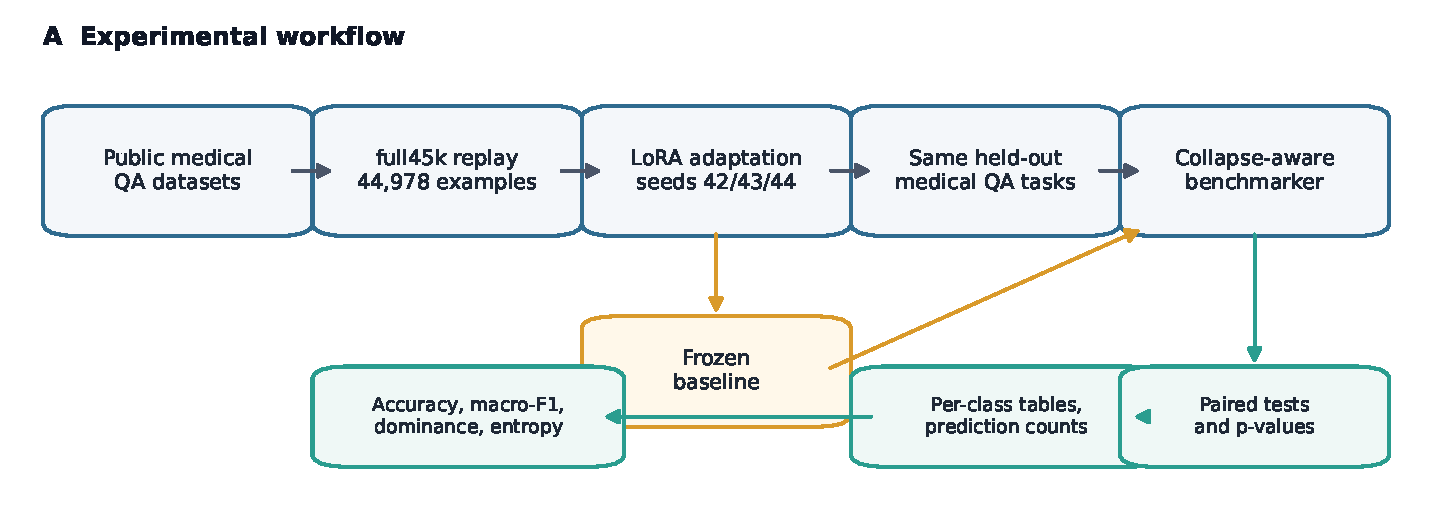
\includegraphics[width=\textwidth]{figures/figure1_pipeline.pdf}
\caption{Experimental workflow. Public medical QA datasets are converted into a full45k replay mixture, evaluated in frozen form, adapted with LoRA self-update, and passed through a collapse-aware benchmarker that reports performance, prediction-distribution, and paired-test statistics.}
\label{fig:pipeline}
\end{figure}

\section{Results}

\subsection{Accuracy Alone Overstates Label-Biased Behavior}

Table~\ref{tab:label_baselines} shows that simple label baselines can obtain non-trivial accuracy while clearly collapsing. The PubMedQA majority baseline always predicts yes and obtains 0.560 accuracy, but macro-F1 is only 0.239 and collapse is flagged. MedMCQA and MedQA majority baselines always predict A and obtain 0.323 and 0.277 accuracy, with macro-F1 scores of 0.122 and 0.109. These results motivate reporting collapse-aware metrics throughout.

\begin{table}[t]
\centering
\small
\caption{Non-model label baselines. Majority baselines are collapsed by construction, even when their accuracy is non-trivial.}
\label{tab:label_baselines}
\begin{tabular}{llllll}
\toprule
Task & Majority label & Majority Acc. & Macro-F1 & Uniform Acc. & Prior Acc. \\
\midrule
PubMedQA & yes & 0.560 & 0.239 & 0.333 & 0.439 \\
MedMCQA & A & 0.323 & 0.122 & 0.250 & 0.260 \\
MedQA & A & 0.277 & 0.109 & 0.250 & 0.253 \\
\bottomrule
\end{tabular}
\end{table}

\subsection{Self-Update Removes Collapse Across Scales}

Table~\ref{tab:main_results} summarizes frozen and full45k results. The 0.5B frozen model collapses on all three tasks. After self-update, collapse decreases from 1/1 to 0/3 runs on each task. PubMedQA accuracy rises from 0.210 to 0.650 $\pm$ 0.046, MedMCQA from 0.317 to 0.414 $\pm$ 0.029, and MedQA from 0.288 to 0.389 $\pm$ 0.023.

The 1.5B model is stronger in frozen form on MedMCQA and MedQA, but still collapses on PubMedQA, with dominant-label rate 0.850. After self-update, PubMedQA collapse is removed in all three seeds, with accuracy 0.690 $\pm$ 0.010 and macro-F1 0.584 $\pm$ 0.040. MedMCQA and MedQA also improve to 0.539 $\pm$ 0.012 and 0.535 $\pm$ 0.010 accuracy.

The 3B model achieves the best MedMCQA and MedQA results, and its three-seed variance is very small: 0.583 $\pm$ 0.003 accuracy on MedMCQA and 0.566 $\pm$ 0.002 on MedQA. However, its frozen PubMedQA behavior still collapses to a maybe-dominant distribution. After self-update, PubMedQA collapse is removed, and accuracy reaches 0.643 $\pm$ 0.031.

\begin{table}[t]
\centering
\scriptsize
\setlength{\tabcolsep}{3.4pt}
\caption{Main frozen-versus-full45k benchmark results. Full45k values are mean $\pm$ standard deviation over three seeds.}
\label{tab:main_results}
\begin{tabular}{llccccc}
\toprule
Task & Model & Frozen Acc. & Full45k Acc. & $\Delta$ Acc. & Full45k F1 & Collapse \\
\midrule
PubMedQA & 0.5B & 0.210 & 0.650 $\pm$ 0.046 & +0.440 & 0.498 $\pm$ 0.063 & 1/1 $\rightarrow$ 0/3 \\
PubMedQA & 1.5B & 0.620 & 0.690 $\pm$ 0.010 & +0.070 & 0.584 $\pm$ 0.040 & 1/1 $\rightarrow$ 0/3 \\
PubMedQA & 3B & 0.230 & 0.643 $\pm$ 0.031 & +0.413 & 0.571 $\pm$ 0.045 & 1/1 $\rightarrow$ 0/3 \\
MedMCQA & 0.5B & 0.317 & 0.414 $\pm$ 0.029 & +0.097 & 0.397 $\pm$ 0.030 & 1/1 $\rightarrow$ 0/3 \\
MedMCQA & 1.5B & 0.436 & 0.539 $\pm$ 0.012 & +0.103 & 0.528 $\pm$ 0.011 & 0/1 $\rightarrow$ 0/3 \\
MedMCQA & 3B & 0.490 & 0.583 $\pm$ 0.003 & +0.093 & 0.576 $\pm$ 0.001 & 0/1 $\rightarrow$ 0/3 \\
MedQA & 0.5B & 0.288 & 0.389 $\pm$ 0.023 & +0.101 & 0.381 $\pm$ 0.024 & 1/1 $\rightarrow$ 0/3 \\
MedQA & 1.5B & 0.470 & 0.535 $\pm$ 0.010 & +0.065 & 0.531 $\pm$ 0.010 & 0/1 $\rightarrow$ 0/3 \\
MedQA & 3B & 0.496 & 0.566 $\pm$ 0.002 & +0.069 & 0.562 $\pm$ 0.002 & 0/1 $\rightarrow$ 0/3 \\
\bottomrule
\end{tabular}
\end{table}

\begin{figure}[t]
\centering
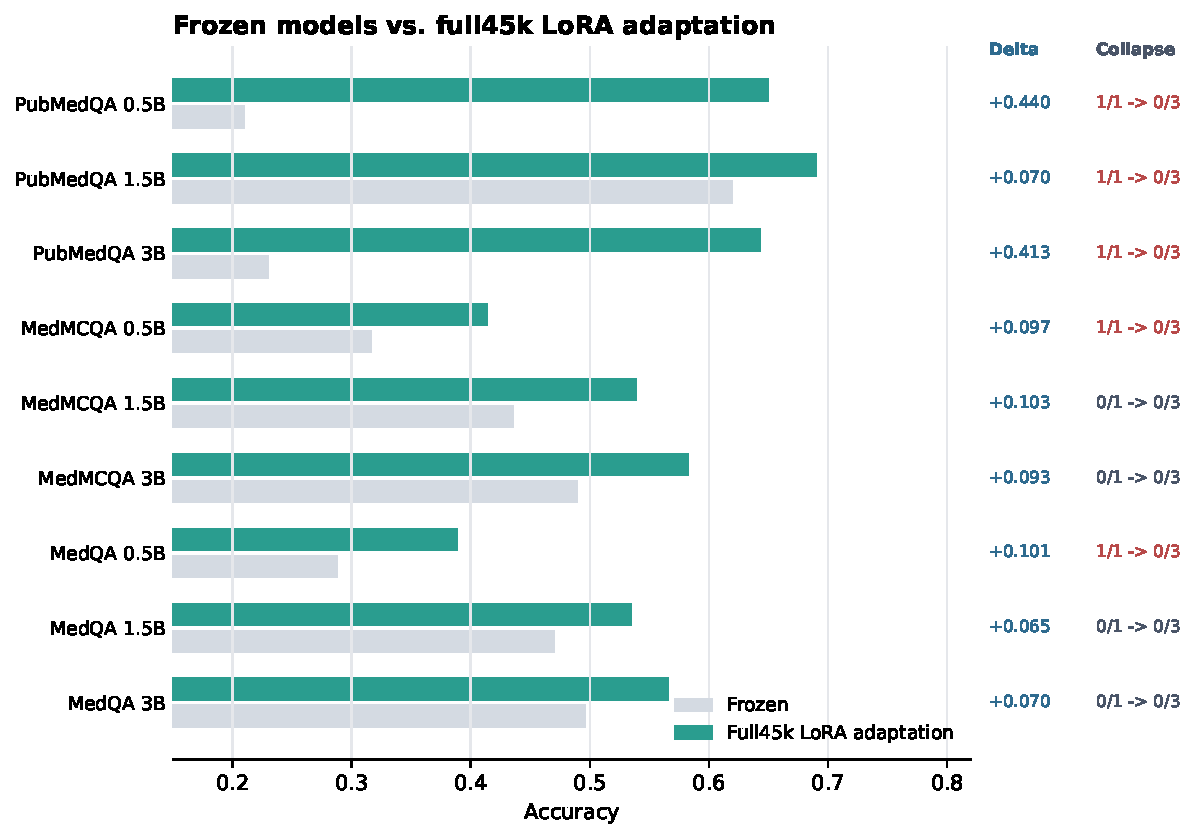
\includegraphics[width=\textwidth]{figures/figure2_results.pdf}
\caption{Paired accuracy changes from frozen evaluation to full45k self-update. Each row compares the same model scale and task before and after LoRA adaptation. Red rings mark collapsed frozen runs; all updated conditions remove collapse across three seeds.}
\label{fig:main_results_plot}
\end{figure}

\subsection{Paired Tests Support Most Accuracy Gains}

Table~\ref{tab:paired_summary} summarizes paired McNemar tests. The 0.5B and 3B models improve significantly across all tasks and seeds. For 1.5B, MedMCQA and MedQA are significant in every seed. PubMedQA improves in accuracy and removes collapse for 1.5B, but paired accuracy tests are not significant; this suggests that the PubMedQA effect for 1.5B should be described as distributional recalibration rather than a statistically significant accuracy gain.

\begin{table}[t]
\centering
\small
\caption{Summary of paired McNemar tests across seeds.}
\label{tab:paired_summary}
\begin{tabular}{llll}
\toprule
Model & Task & $\Delta$ Accuracy Range & Paired Result \\
\midrule
0.5B & PubMedQA & +0.400 to +0.490 & Significant, all seeds \\
0.5B & MedMCQA & +0.064 to +0.115 & Significant, all seeds \\
0.5B & MedQA & +0.076 to +0.121 & Significant, all seeds \\
1.5B & PubMedQA & +0.060 to +0.080 & Not significant \\
1.5B & MedMCQA & +0.092 to +0.115 & Significant, all seeds \\
1.5B & MedQA & +0.058 to +0.077 & Significant, all seeds \\
3B & PubMedQA & +0.380 to +0.440 & Significant, all seeds \\
3B & MedMCQA & +0.091 to +0.096 & Significant, all seeds \\
3B & MedQA & +0.068 to +0.071 & Significant, all seeds \\
\bottomrule
\end{tabular}
\end{table}

\subsection{Scaling Helps, But Not Monotonically}

The scale comparison is task-dependent. On MedMCQA and MedQA, 3B full45k is strongest and has the lowest variance. On PubMedQA, the best result comes from 1.5B, while the 3B frozen baseline collapses despite having better frozen performance on the multiple-choice tasks. This indicates that model scale alone does not guarantee stable answer distributions. Task format and label distribution interact with adaptation dynamics.

\section{Discussion}

The central finding is not simply that full45k improves accuracy. Rather, task-driven self-update changes how small medical language models use the answer space. Frozen small models can behave like biased label predictors: they overuse a dominant label and produce low-entropy outputs. LoRA self-update reduces this behavior, improving macro-F1 and entropy while removing collapse flags.

\begin{figure}[t]
\centering
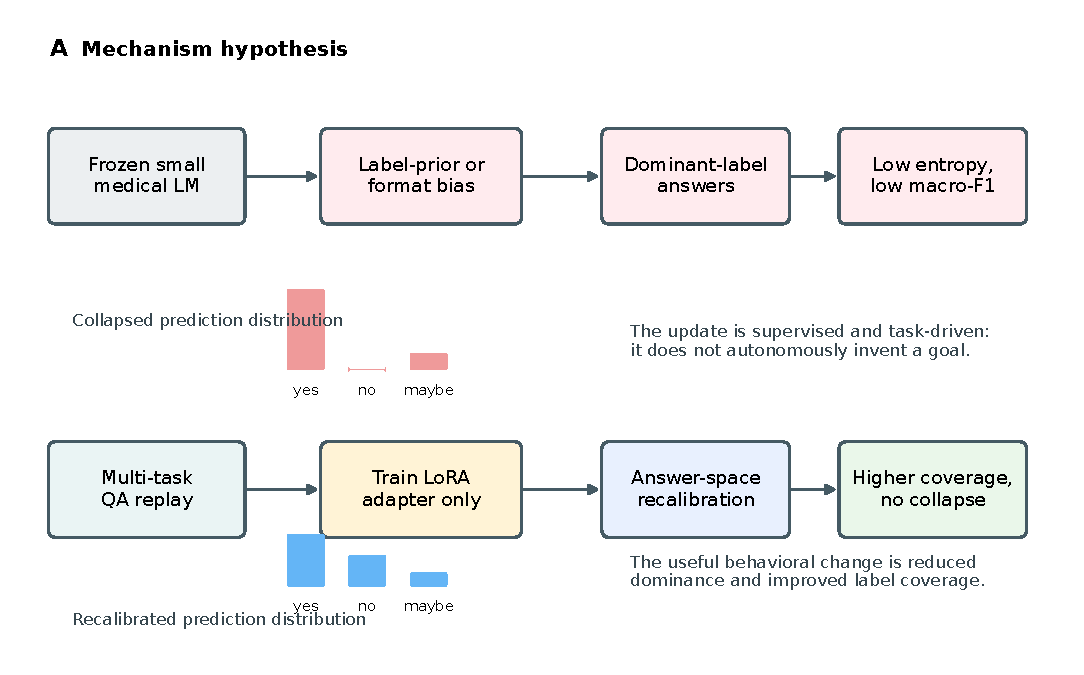
\includegraphics[width=\textwidth]{figures/figure3_mechanism.pdf}
\caption{Mechanism hypothesis. Frozen small medical language models can overuse a dominant answer label because of label-prior or format bias. Task-driven LoRA self-update exposes the model to multi-task QA evidence and recalibrates answer-space usage, reducing dominant-label behavior without claiming autonomous self-improvement.}
\label{fig:mechanism}
\end{figure}

This is particularly important for medical QA evaluation. Accuracy can reward a frequent-label heuristic, especially in small or imbalanced test sets. Collapse-aware reporting makes this visible. For PubMedQA, majority yes already reaches 0.560 accuracy; therefore, a model must be evaluated by how well it handles no and maybe labels, not just by aggregate correctness. For MedMCQA and MedQA, macro-F1 and collapse flags reveal whether the model genuinely covers A/B/C/D choices.

The results also qualify a common scaling intuition. Larger models help substantially on MedMCQA and MedQA, but PubMedQA remains sensitive to label format and uncertainty. The strongest PubMedQA full45k result is from 1.5B rather than 3B. Thus, the useful scientific claim is not ``larger is always better,'' but ``lightweight task-driven updates can mitigate collapse, while task format modulates the effect of scale.''

\section{Limitations}

First, PubMedQA test100 is small, so its accuracy estimates have high uncertainty. We address this partly with three seeds and paired tests, but larger evaluation would strengthen the claim. Second, the study focuses on benchmark QA rather than real clinical deployment; results should not be interpreted as clinical safety evidence. Third, we evaluate LoRA self-update but do not compare against alternative adaptation methods such as full fine-tuning, prompt-only calibration, retrieval augmentation, or class-balanced replay. Fourth, the full45k mixture is fixed; task mixture ratios may affect PubMedQA uncertainty labels, especially maybe. Finally, the work studies final-answer prediction, not explanation quality, factual grounding, or harm avoidance.

\section{Conclusion}

We presented a collapse-aware study of task-driven self-update for resource-limited medical language models. Across Qwen2.5-Instruct 0.5B, 1.5B, and 3B models, LoRA adaptation on a 44,978-example multi-task replay mixture removed answer collapse across PubMedQA, MedMCQA, and MedQA. The strongest multiple-choice results came from 3B with very low variance, while PubMedQA favored 1.5B, showing that scale and task format interact. These results support collapse-aware evaluation as a necessary complement to accuracy when studying small medical language models.

\section*{Declarations}

\paragraph{Funding.}
No specific funding was received for this work.

\paragraph{Competing interests.}
The authors declare that they have no competing interests.

\paragraph{Ethics approval and consent to participate.}
Not applicable. This study used publicly available benchmark datasets and did not involve human participants, human tissue, or identifiable personal information.

\paragraph{Consent for publication.}
Not applicable.

\paragraph{Availability of data and materials.}
PubMedQA, MedMCQA, MedQA, and Qwen2.5-Instruct are publicly available from their original providers. The analysis scripts, aggregate result tables, reproducibility instructions, and manuscript source files are prepared for public release in a GitHub repository: \url{https://github.com/123hzq321/collapse-aware-medical-self-update}.

\paragraph{Authors' contributions.}
Z.H. conceived the study, designed the computational experiments, processed the data, implemented the analysis pipeline, performed model training and evaluation, prepared figures and tables, and drafted the manuscript. X.B. supervised the study, contributed clinical interpretation, and revised the manuscript. Both authors reviewed and approved the final manuscript.

\paragraph{Acknowledgements.}
Not applicable.

\paragraph{Use of AI-assisted tools.}
The authors used AI-assisted language and coding tools during manuscript drafting and code development. The authors reviewed, edited, and verified all content, analyses, and conclusions, and take full responsibility for the submitted work. No AI tool is listed as an author.

\bibliographystyle{plain}
\bibliography{references}

\appendix

\section{Reproducibility Details}

All full45k self-update runs used one epoch, learning rate $2\times10^{-4}$, LoRA rank 8, alpha 16, dropout 0.05, and seeds 42, 43, and 44. The 0.5B and 1.5B runs used 5,623 optimizer steps; the 3B runs used 2,812 optimizer steps. The benchmarker outputs accuracy, macro-F1, dominant-label rate, normalized entropy, collapse flags, prediction counts, label baselines, grouped aggregates, and paired McNemar tests.

\end{document}
